\documentclass[12pt, a4paper, oneside]{article}\usepackage[]{graphicx}\usepackage[]{color}
%% maxwidth is the original width if it is less than linewidth
%% otherwise use linewidth (to make sure the graphics do not exceed the margin)
\makeatletter
\def\maxwidth{ %
  \ifdim\Gin@nat@width>\linewidth
    \linewidth
  \else
    \Gin@nat@width
  \fi
}
\makeatother

\definecolor{fgcolor}{rgb}{0.345, 0.345, 0.345}
\newcommand{\hlnum}[1]{\textcolor[rgb]{0.686,0.059,0.569}{#1}}%
\newcommand{\hlstr}[1]{\textcolor[rgb]{0.192,0.494,0.8}{#1}}%
\newcommand{\hlcom}[1]{\textcolor[rgb]{0.678,0.584,0.686}{\textit{#1}}}%
\newcommand{\hlopt}[1]{\textcolor[rgb]{0,0,0}{#1}}%
\newcommand{\hlstd}[1]{\textcolor[rgb]{0.345,0.345,0.345}{#1}}%
\newcommand{\hlkwa}[1]{\textcolor[rgb]{0.161,0.373,0.58}{\textbf{#1}}}%
\newcommand{\hlkwb}[1]{\textcolor[rgb]{0.69,0.353,0.396}{#1}}%
\newcommand{\hlkwc}[1]{\textcolor[rgb]{0.333,0.667,0.333}{#1}}%
\newcommand{\hlkwd}[1]{\textcolor[rgb]{0.737,0.353,0.396}{\textbf{#1}}}%

\usepackage{framed}
\makeatletter
\newenvironment{kframe}{%
 \def\at@end@of@kframe{}%
 \ifinner\ifhmode%
  \def\at@end@of@kframe{\end{minipage}}%
  \begin{minipage}{\columnwidth}%
 \fi\fi%
 \def\FrameCommand##1{\hskip\@totalleftmargin \hskip-\fboxsep
 \colorbox{shadecolor}{##1}\hskip-\fboxsep
     % There is no \\@totalrightmargin, so:
     \hskip-\linewidth \hskip-\@totalleftmargin \hskip\columnwidth}%
 \MakeFramed {\advance\hsize-\width
   \@totalleftmargin\z@ \linewidth\hsize
   \@setminipage}}%
 {\par\unskip\endMakeFramed%
 \at@end@of@kframe}
\makeatother

\definecolor{shadecolor}{rgb}{.97, .97, .97}
\definecolor{messagecolor}{rgb}{0, 0, 0}
\definecolor{warningcolor}{rgb}{1, 0, 1}
\definecolor{errorcolor}{rgb}{1, 0, 0}
\newenvironment{knitrout}{}{} % an empty environment to be redefined in TeX

\usepackage{alltt} % Paper size, default font size and one-sided paper
%\graphicspath{{./Figures/}} % Specifies the directory where pictures are stored
%\usepackage[dcucite]{harvard}
\usepackage{rotating}
\usepackage{amsmath}
\usepackage{setspace}
\usepackage{pdflscape}
\usepackage[flushleft]{threeparttable}
\usepackage{multirow}
\usepackage{tikz}
\usepackage[comma, sort&compress]{natbib}% Use the natbib reference package - read up on this to edit the reference style; if you want text (e.g. Smith et al., 2012) for the in-text references (instead of numbers), remove 'numbers' 
\usepackage{graphicx}
%\bibliographystyle{plainnat}
\bibliographystyle{agsm}
\usepackage[colorlinks = true, citecolor = blue, linkcolor = blue]{hyperref}
%\hypersetup{urlcolor=blue, colorlinks=true} % Colors hyperlinks in blue - change to black if annoying
%\renewcommand[\harvardurl]{URL: \url}
 \usepackage{listings}
 \usepackage{color}
 \graphicspath{{../Pictures/}}
\definecolor{mygrey}{gray}{0.95}
\lstset{backgroundcolor=\color{mygrey}}
\IfFileExists{upquote.sty}{\usepackage{upquote}}{}
\begin{document}
\title{Calculus}
\author{Rob Hayward}
%\date{\today}
\maketitle
%\begin{abstract}
%erehrere
%\end{abstract}
\section*{Introduction}
\begin{itemize}
\item Economics is all about relationships
\begin{itemize}
\item tax - spend
\item education - income
\item R and D - Sales
\end{itemize}

\item We would like to measure these relationships
\end{itemize}

Take the following equation
\begin{equation*}
Q_d = 25 - 2P
\end{equation*}

\begin{knitrout}
\definecolor{shadecolor}{rgb}{0.969, 0.969, 0.969}\color{fgcolor}
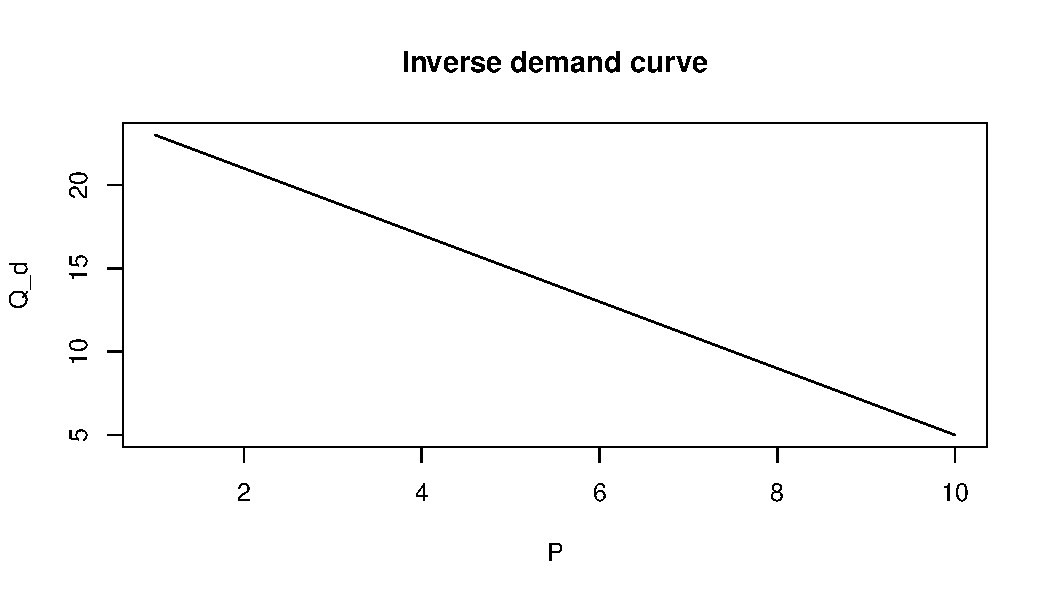
\includegraphics[width=\maxwidth]{figure/demand-1} 

\end{knitrout}
Remember that the elasticity is calculated as 
\begin{align*}
\varepsilon_d =& \frac{Q_2 - Q_1}{Q1}/\frac{P_2 - P_1}{P_1}\\
          =& \frac{Q_2 - Q_1}{Q_1} \times \frac{P_1}{P_2 - P_1}\\
          =& \frac{\Delta(Q) P_1}{\Delta(P) Q_1}
\end{align*}

Knowing that $\Delta(Q)/\Delta(P) = -5$, this rule can be applied to any point on the graph.

For example, when $P = 6, Q = 13$ and the elasticity of demand at that point is 

\begin{align*}
\varepsilon_d =& -5 \times \frac{6}{13}\\
              =& -2.3077
\end{align*}

That is all very well, but what happens when there are non-linear relationships?  The last elasticity examples that we looked at had a non-linear demand curve. 

\begin{equation} 
Q_d = 50 -15P + P^2
\end{equation}
\begin{knitrout}
\definecolor{shadecolor}{rgb}{0.969, 0.969, 0.969}\color{fgcolor}
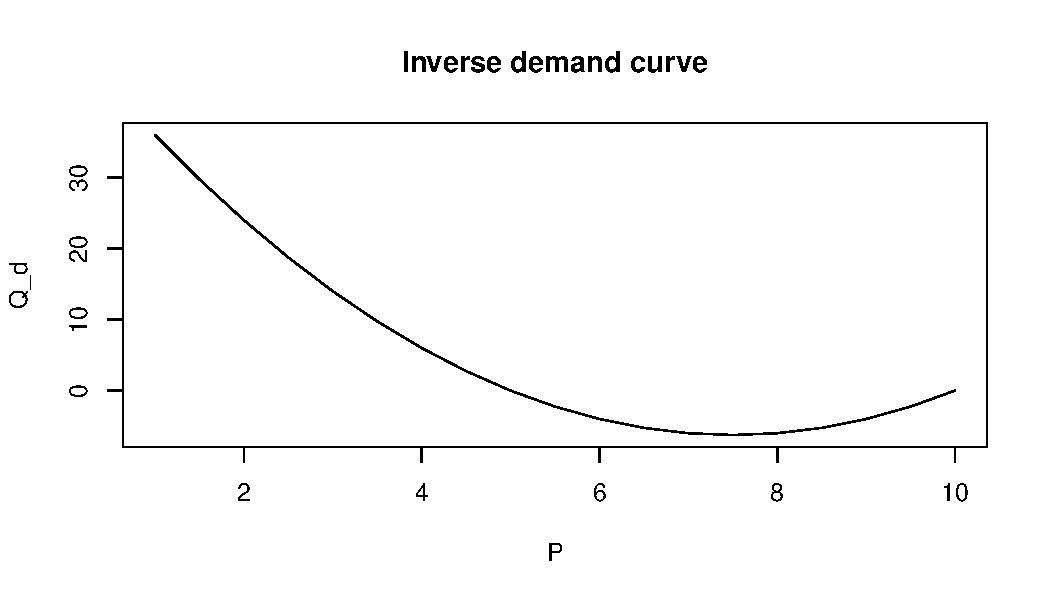
\includegraphics[width=\maxwidth]{figure/demand2-1} 

\end{knitrout}
\subsection{Usain Bolt}

\begin{tikzpicture}[xscale = 1, yscale = 1/10, scale = 0.8]
\draw [thick, <->] (0,100) -- (0,0) -- (10,0);
\draw [thin] (0,0) -- (9.58, 100);
\node [below left] at (9,0) {x = seconds};
\node [above, rotate = 90] at (0,95) {y = meters};
\draw [<->, blue] (0,0) to [out = 57, in = 232] (9.58, 100);
\node [below right] at (9.58, 100) {UB};
\end{tikzpicture}

The average speed can be calculated as the total distance divided by the time
\begin{equation*}
\text{average speed} = \frac{\text{total distance}}{\text{total time}}
\end{equation*}

In this case, that is 
\begin{equation*}
\text{average speed} = \frac{\text{100 meters}}{\text{9.58 seconds}}
\end{equation*}

This is $10.43\frac{m}{s}$
However, if you want the instantaneous speed, it is necessary to draw the line at a tangent to the curve. 






\end{document}
